
\chapter{Benutzeroberfläche}
\begin{itemize}
\item Das Hauptelement der Benutzeroberfläche ist die Karten- oder Globusansicht, die sich im rechten Fensterteil befindet. Der sichtbare Kartenausschnitt kann interaktiv mit Maus oder Tastatur verschoben werden.
\item Im 2D-Modus zeigt die Ansicht eine Projektion der Karte auf die Ebene, die in der Ansicht nach links/rechts und oben/unten verschoben sowie (perspektivisch) gekippt werden kann.
\item Im 3D-Modus wird ein Globus gezeigt, auf den das Kartenmaterial projiziert wird. Die Ansicht kann um die Erdachse sowie in Richtung der Pole gedreht; ab einem gewissen Zoomlevel am Kameraursprung gekippt werden.
\item Am linken Rand des Fensters befindet sich eine Seitenleiste, die sämtliche Steuerungsfunktionen bereitstellt. Sie ist in Tabs unterteilt, mit denen die Funktionen gruppiert werden.
\end{itemize}
\begin{figure}
	\centering
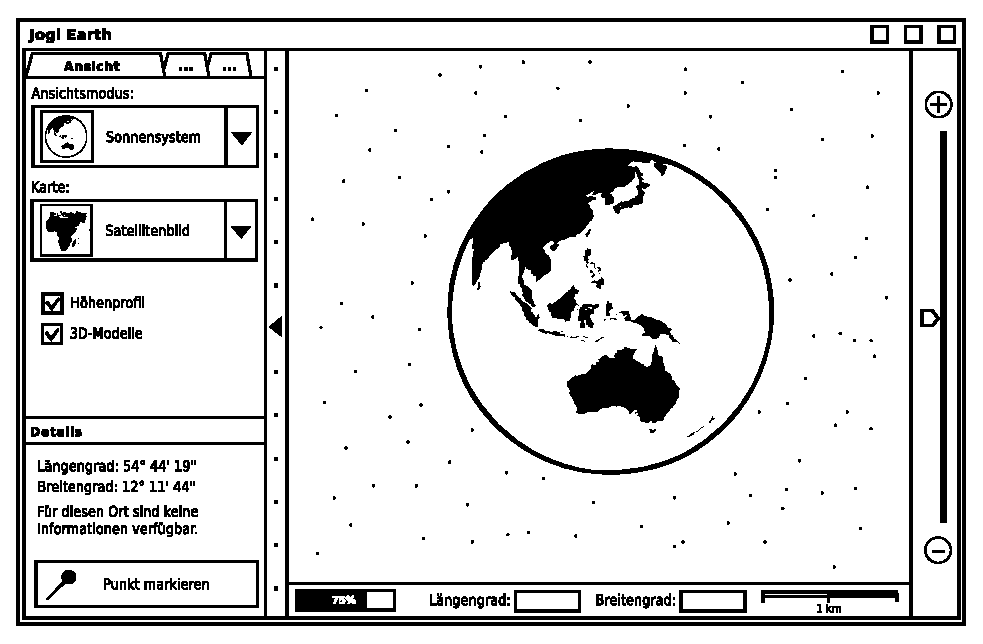
\includegraphics[scale=0.9]{GUI-Ansicht.eps}
	\caption{Die Benutzeroberfläche mit geöffnetem Ansichts-Tab}
\end{figure}
\begin{figure}
	\centering
\begin{minipage}[c]{5cm}
	\centering
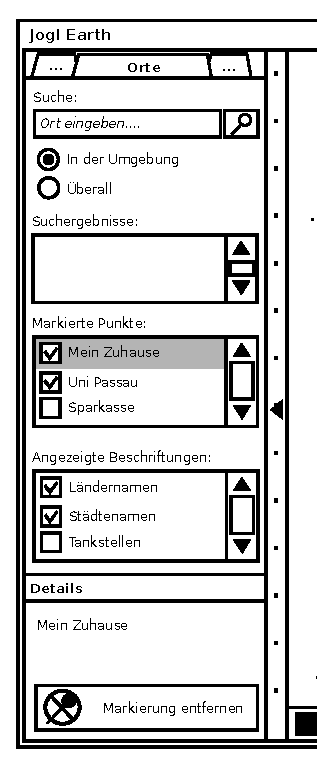
\includegraphics[scale=0.9]{GUI-Orte.eps}
\end{minipage}
	\caption{Bild2}
	\label{Bild2}
\begin{minipage}[c]{5cm}
	\centering
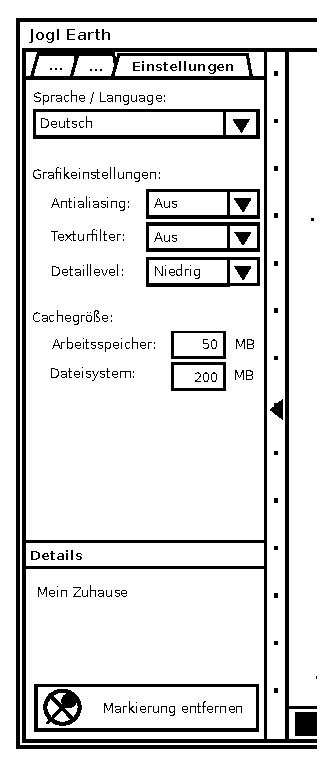
\includegraphics[scale=0.9]{GUI-Einstellungen.eps}
\end{minipage}
	\caption{Bild2}
	\label{Bild2}
	\end{figure}